
% Preámbulo

\documentclass[12pt,a4paper,oneside,english,spanish, donotrepeattitle, floatsintext, natbib]{TesisUNSCH}

    \usepackage[utf8]{inputenc}
\usepackage{comment}
\usepackage{marvosym}
\usepackage{graphicx}
\usepackage[natbibapa]{apacite} %Agregar formato de citación APA
\bibliographystyle{apacite}
\setlength{\bibsep}{5pt plus 0.3ex} %Espaciamiento en la bibliografía
\setcounter{secnumdepth}{3} % Numera los secciones
\usepackage[T1]{fontenc}
\usepackage[normalem]{ulem}
\usepackage[spanish, es-tabla]{babel} %% reemplaza "cuadro" por "tabla"
\useunder{\uline}{\ul}{}
\newcommand{\myparagraph}[1]{\paragraph{#1}\mbox{}\\}
\decimalpoint  %Cambia coma por punto
\usepackage{mathptmx}
\usepackage{layouts} %Saber ancho de hoja.
\usepackage{fontspec}
\usepackage{amssymb}
\usepackage{changepage} %Agregar identación
\setmainfont{Arial}
\usepackage{setspace}
\usepackage[left=3.81 cm,right=2.54 cm,top=2.54 cm,bottom=2.54 cm]{geometry}
%\usepackage{fancyhdr} %Encabezado y Pie de página (1)
%\pagestyle{fancy} %Encabezado y Pie de página (2)
\usepackage{lipsum} %Crear texto RAMDOM
\renewcommand{\labelitemi}{$\bullet$} %Circulos para viñetas
\usepackage{titlesec} %Titulos de SECCIONES
\usepackage{tocloft} %Titulos de ÍNDICES
\usepackage[colorlinks=true,linkcolor=negro,citecolor = negro]{hyperref}
\usepackage[mathbf=sym]{unicode-math} % Mantener fuentes matemáticas
\makeatletter  %Comando para REDUCIR ERRORES
\usepackage{multirow} % Agregar TABLAS 
\usepackage{array} % Dar formato a las TABLAS
\usepackage{subcaption} % Insertar SubImagenes
\usepackage{tikz} % Diagrama de Flujo
\usetikzlibrary{calc,positioning,shapes.geometric,shapes.symbols,shapes.misc}

% Insertar formas para diagramas de flujo
\tikzstyle{startstop} = [rectangle, rounded corners, minimum width=3cm, minimum height=0.5cm,text centered, draw=black]
\tikzstyle{io} = [trapezium, trapezium left angle=70, trapezium right angle=110, minimum width=3cm, minimum height=0.5cm, text centered, text width=3cm, draw=black]
\tikzstyle{process} = [rectangle, minimum width=3cm, minimum height=0.5cm, text centered, text width=4cm, draw=black]
\tikzstyle{decision} = [diamond, minimum width=3cm, minimum height=0.5cm, text centered, draw=black]
\tikzstyle{loop} = [chamfered rectangle,chamfered rectangle xsep=2cm,draw=black]
\tikzstyle{arrow} = [->,>=stealth]
\tikzstyle{line}=[draw]

\usepackage{listings}
\usepackage{color}

%New colors defined below
\definecolor{codegreen}{rgb}{0,0.6,0}
\definecolor{codegray}{rgb}{0.5,0.5,0.5}
\definecolor{codepurple}{rgb}{0.2,0,1}
\definecolor{codeRojo}{rgb}{0.7,0,0.3}
\definecolor{backcolour}{rgb}{1.0, 1.0, 1.0}

%Code listing style named "mystyle"
\lstdefinestyle{mystyle}{
  backgroundcolor=\color{backcolour},  
  commentstyle=\color{codegreen},
  keywordstyle=\color{codeRojo},
  numberstyle=\tiny\color{codegray},
  stringstyle=\color{codepurple},
  basicstyle=\footnotesize,
  breakatwhitespace=false,         
  breaklines=true,                 
  captionpos=b,                    
  keepspaces=true,                 
  numbers=left,                    
  numbersep=5pt,                  
  showspaces=false,                
  showstringspaces=false,
  showtabs=false,                  
  tabsize=2
}

%"mystyle" code listing set
\lstset{style=mystyle}

\newenvironment{MyFont}{\fontfamily{ugm}\selectfont}{\par}

\usepackage{changepage} %Agregar espacio a Listing



% Centrado del título del ÍNDICE / LISTA DE FIGURAS / LISTA DE CUADROS

\renewcommand{\cfttoctitlefont}{\hfill \normalfont\normalsize\bfseries}
\renewcommand{\cftaftertoctitle}{\hfill}

\renewcommand{\cftlottitlefont}{\hfill\normalfont\normalsize\bfseries}
\renewcommand{\cftafterlottitle}{\hfill}

\renewcommand{\cftloftitlefont}{\hfill\normalfont\normalsize\bfseries}
\renewcommand{\cftafterloftitle}{\hfill}


% Formato de los CAPÍTULOS, SECCIONES Y SUBSECCIONES
\titleformat{\chapter}[block]{\normalfont\normalsize\bfseries}{CAPÍTULO \thechapter:}{0.5em}{\normalsize}
\titlespacing*{\chapter}{0pt}{-10 pt}{5pt}

\titleformat{\section}[block]{\normalfont\normalsize}{\thesection}{0.5em}{\normalsize}
\titlespacing*{\section}{0pt}{10 pt}{5 pt}

\titleformat{\subsection}[block]{\normalfont\normalsize}{\thesubsection}{0.5em}{\normalsize}
\titlespacing*{\subsection}{0pt}{10 pt}{5 pt}

\titleformat{\subsubsection}[block]{\normalfont\normalsize}{\thesubsubsection}{0.5em}{\normalsize}
\titlespacing*{\subsubsection}{0pt}{10 pt}{5 pt}


% Espaciado entre PÁRRAFOS y SANGRÍA
\setlength{\parskip}{5 pt}
\setlength{\parindent}{0cm}


% Dar formato a las TABLAS
\newcolumntype{M}[1]{>{\centering\arraybackslash}m{#1}}
\newcolumntype{L}[1]{>{\raggedright\arraybackslash}m{#1}}
\newcolumntype{R}[1]{>{\raggedleft\arraybackslash}m{#1}}
\newcolumntype{N}{@{}m{0pt}@{}}
\renewcommand{\arraystretch}{1.25}

% Cambiar titulo de bibliografía
\addto\captionsspanish{\renewcommand{\bibname}{\centering REFERENCIAS BIBLIOGRÁFICAS}}


% Posicionamiento vertical de TOC, LOT and LOF

\setlength{\cftbeforelottitleskip}{1pt} 
\renewcommand{\cftafterlottitleskip}{12pt}

\setlength{\cftbeforeloftitleskip}{1pt} 
\renewcommand{\cftafterloftitleskip}{12pt}

\setlength{\cftbeforetoctitleskip}{16pt} 
\renewcommand{\cftaftertoctitleskip}{12 pt}


% Cambiando las etiquetas de las FIGURAS y TABLAS (Caption y autoref)
\addto\captionsspanish{\renewcommand{\figurename}{\footnotesize FIGURA N°}}
\addto\extrasspanish{\def\figureautorefname{ Figura N°}}
 
\addto\captionsspanish{\renewcommand{\tablename}{\footnotesize TABLA N°}}
\addto\extrasspanish{\def\tableautorefname{ Tabla N°}} 


% Espaciamiento dentro del índice

\setlength{\cftbeforechapskip}{2mm}
\renewcommand\cftchapafterpnum{\vskip6pt}
\renewcommand\cftsecafterpnum{\vskip5pt}
\renewcommand\cftsubsecafterpnum{\vskip5pt}


%Agregar la palabra CAPITULO al TOC, FIGURA a LOF y TABLA al LOT

\renewcommand{\cftchappresnum}{CAPÍTULO }
\renewcommand{\cftchapaftersnum}{:}
\renewcommand{\cftchapnumwidth}{7em}

\renewcommand{\cftfigpresnum}{Figura N° }
%\renewcommand{\cftfigaftersnum}{:}
\renewcommand{\cftfignumwidth}{6.85 em}

\renewcommand{\cfttabpresnum}{Tabla N° }
%\renewcommand{\cftfigaftersnum}{:}
\renewcommand{\cfttabnumwidth}{6.5 em}


%Definición de COLORES

\usepackage{xcolor}
\definecolor{granate}{RGB}{113,22,16}
\definecolor{gris}{RGB}{154,153,157}
\definecolor{arena}{RGB}{230,217,170}
\definecolor{azul}{rgb}{0.03, 0.15, 0.4}
\definecolor{negro}{rgb}{0, 0, 0}

%Cambiando a Números Romanos los Capítulos
\renewcommand{\thesection}{\Roman{section}} %Las secciones estaran con numeración romana MAYUSCULA
\renewcommand{\thesubsection}{\arabic{section}.\arabic{subsection}}  
\renewcommand{\theequation}{\arabic{section}.\arabic{equation}} 
\renewcommand{\thetable}{\arabic{section}.\arabic{table}}  
\renewcommand{\thefigure}{\arabic{section}.\arabic{figure}}


%Escribir los INFORMACIÓN PERSONAL Y DEL TRABAJO

%Autor para PIE DE PÁGINA (Respetar mayusculas y minisculas)
\author{Elmer Edison ACHALMA MENDOZA y Kattya Yashitrh CASTILLO LOPEZ}

%Autor para CARÁTULA (Siempre en mayuscula y sin saltos de linea)
\authorcaratula{Elmer Edison ACHALMA MENDOZA \\[2mm] Kattya Yashitrh CASTILLO LOPEZ}

%Título en para el PIE DE PÁGINA (Agregar salto de línea de ser necesario)
\title{Crecimiento económico y pobreza en el departamento Ayacucho, periodo 2000-2019}

%Título para CARÁTULA (Siempre en mayuscula y sin saltos de linea)
\titlecaratula{Crecimiento económico y pobreza en el departamento Ayacucho, periodo 2000-2019}

%Nombre de la FACULTAD (Siempre en mayuscula)
\facultad{FACULTAD DE CIENCIAS ECONÓMICAS, ADMINISTRATIVAS Y CONTABLES}

%Para obtener el título profesional de ... (Siempre en mayuscula)
\grado{Economista}

%Asesor para CARÁTULA (Siempre en mayuscula y sin saltos de linea)
\asesor{Dr. Pelayo HILARIO VALENZUELA}

%AÑO para CARÁTULA
\yyearr{2021}



\begin{document}
	
	\renewcommand{\BOthers}[1]{et al.\hbox{}} %Agregar et al.
	\onehalfspacing 	% Interlineado 1.5
	\noindent			% Sin sangría
		
	%Parte INCIAL DE LA TESIS
	
	\frontmatter 
		
	\begin{titlepage}
	
	\begin{center}
		\vspace*{\baselineskip}
        {
		{\normalsize  \textrm{UNIVERSIDAD NACIONAL SAN CRISTÓBAL DE HUAMANGA}}\\
		\vspace{5 mm}
		{\small \textrm{\@facultad}}\\
		\vspace{5 mm}
		{\large \textrm{ESCUELA PROFESIONAL DE ECONOMÍA}}\\
		}
		\vspace*{0.5\baselineskip}
		
		\begin{figure}[h]
			\centering 
			{
\includegraphics[width=0.3\textwidth]{E. Imágenes/0. Caratula/Logo}\par}
		\end{figure}
		
		\vspace{1 mm}	

		\onehalfspacing  % Espaciamiento 1.5
		{\Large \textbf{\@titlecaratula}}\\
		
		\singlespacing  % Fin del espaciamiento 1.5
		
		\vspace{5 mm}
		{\large \textbf{Proyecto de Tesis} }\\
		\vspace{5 mm}	
		%{\large{Para optar Grado Académico de Bachiller en Ciencias Económicas Mención {\@grado} } }\\
		%\vspace{10 mm}
		{\large \textsl{Presentado por:} }\\
		\vspace{5 mm}	
		{\Large{\@authorcaratula}}\\
		\vspace{10 mm}
		{\large \textsl{Asesor:} } {\large \textsl{\@asesor}}\\
		
		\vfill	
		
		{\large{Ayacucho - Perú} }\\
		\vspace{5 mm}	
		{\large{Octubre, \@yyearr} }\\

	\end{center}

\end{titlepage}
	
	\begin{permisos}

	\onehalfspacing  % Espaciamiento 1.5
	
	© 2021, Universidad Nacional San Cristóbal de Huamanga. Todos los derechos reservados \\
	\textbf{``El autor autoriza a la UNSCH a reproducir la tesis en su totalidad o en parte, con fines estrictamente académicos.''} \\
	Achalma Mendoza, Elmer Edison \\
	Castillo Lopez, Kattya Yashitrh \\
	elmer.achalma.09@unsch.edu.pe \\
	kattya.castillo.09@unsch.edu.pe \\
	934179301 
	
	\singlespacing  % Fin del espaciamiento 1.5
	
\end{permisos}


	\begin{dedication}

Aquí va la dedicatoria\\
a tus padres, hermanos, amigos, etc.

\end{dedication}
	
	\begin{agradecimientos}
\vspace{50 mm}
\normalsize\textbf{\centerline {AGRADECIMIENTOS}} \\

\lipsum[17]

\lipsum[11]


\end{agradecimientos}
	
	%Cambiar nombre y crear ÍNDICE
	\singlespacing 
	\renewcommand\contentsname{\centering ÍNDICE }
	\tableofcontents	
	\onehalfspacing
	
	\cleardoublepage\phantomsection\addcontentsline{toc}{section}{\bf RESUMEN}
\section*{\centerline {RESUMEN}}
\markboth{RESUMEN}{}

\lipsum[5] 


		
	\cleardoublepage\phantomsection\addcontentsline{toc}{section}{\bf {ABSTRACT}}
\section*{\centerline {ABSTRACT}}
\markboth{ABSTRACT}{}

\lipsum[5]

	\cleardoublepage\phantomsection\addcontentsline{toc}{section}{\bf {PRÓLOGO}}
\section*{\centerline {PRÓLOGO}}
\markboth{PRÓLOGO}{}

\lipsum[6] \\ [2mm]
\lipsum[10] 

 
	
	%Cambiar nombre, crear ÍNDICE DE FIGURAS Y TABLAS
	
	\renewcommand\listfigurename{\centering LISTA DE FIGURAS}
	\renewcommand\listtablename{\centering LISTA DE TABLAS}

	\cleardoublepage\phantomsection\addcontentsline{toc}{section}{\bf \listtablename}
	{\normalsize\listoftables}
		
	\cleardoublepage\phantomsection\addcontentsline{toc}{section}{\bf \listfigurename}
	{\normalsize\listoffigures}
	
	\cleardoublepage\phantomsection\addcontentsline{toc}{section}{\bf {LISTA DE SÍMBOLOS Y SIGLAS}}	
\section*{\centerline {LISTA DE SÍMBOLOS Y SIGLAS}}
\markboth{LISTA DE SÍMBOLOS Y SIGLAS}{}
%---
	\section*{\textbf{\underline{SÍMBOLOS}}}

\begin{tabular}{L{0.5 cm}p{0.025 cm}p{12.5 cm}}
$\alpha$           & : & Razón entre la rigidez postfluencia y la   rigidez elástica \\
$A$                & : & Área de la sección transversal de la viga                                                  \\
$\beta$            & : & Porcentaje de amortiguamiento crítico de la superestructura                                \\
$\beta_{a}$        & : & Fracción de amortiguamiento crítico del AMS                                                \\
$\beta_{M}$        & : & Amortiguamiento efectivo de la edificación aislada                                         \\
$B_{M}$            & : & Factor de reducción asociado al amortiguamiento efectivo   $\beta_{M}$                     \\
$c_{a}$            & : & Amortiguamiento del AMS                                                                     
\end{tabular}






	\newpage
	\section*{\textbf{\underline{SIGLAS}}}

\begin{tabular}{L{1.0 cm}p{0.025 cm}p{11.7 cm}}
ADAS    & : & Added damping and stiffness                                                    \\
AMS     & : & Amortiguador de masa sintonizada                                               \\
AS      & : & Aislador sísmico                                                               \\
ASCE    & : & American society of civil engineers                                            
\end{tabular}\\



 
	%Parte CENTRAL DE LA TESIS
	
	\mainmatter 

	% I. PLANTEAMIENTO DEL PROBLEMA
	\section{PLANTEAMIENTO DEL PROBLEMA}
\markboth{CAPÍTULO \thesection: PLANTEAMIENTO DEL PROBLEMA}{}
	
	\subsection{Enunciado del problema}

La desigualdad económica es el distinto reparto de los ingresos, los activos o el bienestar entre el conjunto de habitantes, según explica la Organización para la Cooperación y el Desarrollo Económicos (OECD, 2018).\\
América Latina es la región más desigual de la región en términos socioeconómicos según Nora, L (2011) “la región latinoamericana es 19\% más desigual que el África subsahariana, 37 más desigual que el este asiático y 65\% más desigual que los países desarrollados”.  En efecto América Latina es, hoy, la región sin guerras más desigual del planeta: más que India, más que algunos países de África Subsahariana.\\
La región de América Latina y el Caribe es, según Oxfam, la más desigual en ingresos en el mundo, ya que en 2014 el 1 \% más rico poseía el 41 \% de la riqueza regional, mientras que el 99 \% restante debía repartirse el 60 \%.\\
La desigualdad socioeconómica impide luchar contra la pobreza, ampara que colectivos vulnerables vivan en condiciones de pobreza sin acceso a empleos dignos, servicios básicos, exponiéndose a una dieta pobre o sin una vivienda decente, se prolonga la exclusión y marginación social de personas y familias. \\
En este sentido es evidente la importancia de entender la pobreza.
Ravallion, G. (1991) afirma que la pobreza alude a niveles de vida.  Esto es: ¿cuántas personas no pueden satisfacer ciertas necesidades predeterminadas de consumo y acceso amplio a bienes públicos (servicios de salud, educación, vivienda)?  \\
Según INEI “La pobreza es una condición en la cual una o más personas tienen un nivel de bienestar inferior al mínimo socialmente aceptado.”\\
Las estadísticas indican que desde el año 2000 se ha conseguido reducir la tasa de incidencia de la pobreza en el Perú. \\
El siguiente cuadro del Banco Mundial presenta la tasa de incidencia de la pobreza, sobre la base de la línea de pobreza nacional (\% de la población) para el periodo 2004 – 2019.\\








Donde precisa que la tasa de incidencia de la pobreza entre 2004 y 2019 se redujo en 38.5\%. señala también que el principal periodo de reducción fue entre 2004 y 2011. \\ 
Entre el 2002 y 2016 la pobreza bajo de 54,30 a 20,7\% y la extrema pobreza de 24.2\% a 3.8\%, lo cual indica que en el gobierno de Alejandro Toledo la pobreza disminuyó en 5,2\% y la extrema pobreza en 10,4\%, en el gobierno de Alan García la pobreza se redujo en 21,4\% y la extrema pobreza en 7,5\%; y en el gobierno de Ollanta Humala la pobreza en 7,03\% y la extrema pobreza 2,54\%, llegando en el año 2018 al 20,50\% de pobreza y 2,8\% la extrema pobreza, con tendencia a seguir disminuyendo. \\
En nuestro país la pobreza pasó de 54\% (1990) a 20,50\% (2018) y la extrema pobreza de 24.2\% (1990) a 2.8\% (2018), disminuyendo significativamente en 33,5\% la pobreza y la extrema pobreza en 21.4\%, como consecuencia del crecimiento económico sostenido, el incremento del gasto social, la mejor calidad y focalización de los programas sociales, y el incremento de la inversión pública. \\
En el período 2001-2010, la pobreza decreció en 23,5 puntos porcentuales, al pasar de 54,8\% a 31,3\% en el 2010. \\
Donde precisa que la tasa de incidencia de la pobreza entre 2004 y 2019 se redujo en 38.5\%. señala también que el principal periodo de reducción fue entre 2004 y 2011. \\
Entre el 2002 y 2016 la pobreza bajo de 54,30 a 20,7\% y la extrema pobreza de 24.2\% a 3.8\%, lo cual indica que en el gobierno de Alejandro Toledo la pobreza disminuyó en 5,2\% y la extrema pobreza en 10,4\%, en el gobierno de Alan García la pobreza se redujo en 21,4\% y la extrema pobreza en 7,5\%; y en el gobierno de Ollanta Humala la pobreza en 7,03\% y la extrema pobreza 2,54\%, llegando en el año 2018 al 20,50\% de pobreza y 2,8\% la extrema pobreza, con tendencia a seguir disminuyendo. \\
En nuestro país la pobreza pasó de 54\% (1990) a 20,50\% (2018) y la extrema pobreza de 24.2\% (1990) a 2.8\% (2018), disminuyendo significativamente en 33,5\% la pobreza y la extrema pobreza en 21.4\%, como consecuencia del crecimiento económico sostenido, el incremento del gasto social, la mejor calidad y focalización de los programas sociales, y el incremento de la inversión pública.\\
En el período 2001-2010, la pobreza decreció en 23,5 puntos porcentuales, al pasar de 54,8\% a 31,3\% en el 2010.







En el año 2017, el 21,7\% de la población del país, que equivale en cifras absolutas a 6 millones 906 mil personas, se encontraban en situación de pobreza, es decir, tenían un nivel de gasto inferior al costo de la canasta básica de consumo compuesto por alimentos y no alimentos. Al comparar estos resultados con el nivel obtenido en el año 2016, se observa que la pobreza aumentó en 1,0 p.p, que equivale a 375 mil personas pobres, más que en el año 2016. \\






En el año 2019, el índice de pobreza monetaria afectó al 20,2\% de la población del país, con lo cual mantiene prácticamente los mismos niveles del año 2018; así lo dio a conocer el Instituto Nacional de Estadística e Informática (INEI) según los resultados de la Encuesta Nacional de Hogares (ENAHO) del año 2019. Asimismo, precisó que se considera población en condición de pobreza aquella cuyo gasto per cápita es inferior al valor de la Línea de Pobreza (LP), que es el equivalente monetario de una canasta básica de consumo alimentario y no alimentario. \\
Cuando se habla de pobreza también se hace referencia a la desigualdad social; un grupo social que es excluido ya que no cuenta con el mismo acceso a los recursos que otros grupos con poder si tienen, estas diferencias están marcadas con claridad entre las zonas urbanas y rurales. 
La aplicación errada de políticas públicas ha pronunciado aún más las diferencias, ya que no se ha permitido una integración de la multiculturalidad con la que cuenta el Perú, y muy por el contrario ha ocasionado un marcado distanciamiento entre ellos. \\
En un contexto de crecimiento económico sostenido, es necesario mejorar la formulación y aplicación de las políticas del país, en objetivos puntuales de desarrollo y asistencia social con el firme objetivo de hacerle frente a la pobreza y en un largo plazo mejorar los estándares de vida de su población en conjunto.




	\input{2. 01. Planteamiento del problema/1.2. Formulación del problema.tex}

	



	
	% II. OBJETIVOS
	\section{OBJETIVOS}
\markboth{CAPÍTULO \thesection: MARCO TEÓRICO Y CONCEPTUAL}{}

	\subsection{Objetivo general}

Establecer cómo de la desigualdad socioeconómica incide en la pobreza en el departamento de Ayacucho, periodo 2000-2019.

	
	
	


	\input{2. 02. Objetivos/2.2. Objetivos específicos.tex}
	
	


	
		
	% III. JUSTIFICACIÓN
	\section{JUSTIFICACIÓN}
\markboth{CAPÍTULO \thesection: JUSTIFICACIÓN}{}

	\subsection{Justificación teórica}
	
La pobreza es un problema mundial que se ha venido combatiendo a lo largo de los años, cada país en forma individual ha implementado medidas y políticas con el único fin de reducir su nivel de pobreza o extrema pobreza. En caso particular de Perú, a pesar de los índices favorables en la reducción de la pobreza, en determinadas zonas se observa un margen significativo en la desigualdad socioeconómica el cual es paralelo al índice del nivel pobreza.\\
Es importante analizar el comportamiento de los índices de pobreza contrastado con indicadores de la desigualdad socioeconómica; para así poder establecer un grado de eficacia o trascendencia en el tiempo. Generar conocimiento en la relación que se establecen entre estos indicadores, de manera que se contraste con la teoría económica ya conocida o se generen nuevos aportes.


	\subsection{Justificación practica}


Este trabajo tiene una justificación practica porque con él podrá ser posible su aplicación a la realidad para poder hacer frente a la desigualdad socioeconómica que predomina en distintas regiones en particular y sobre todo hacer frente a la pobreza que tanto sufrimiento ocasiona a una gran parte de la población peruana. \\
Los resultados de la presente investigación podrán aportar a ver mejor el panorama del país y con él se podrán diseñar estrategias de políticas públicas con los que en un mediano plazo podamos obtener resultados más eficaces en la reducción de la pobreza y la desigualdad socioeconómica en el Perú; además del gran aporte que significara para la toma de decisiones a nivel de gobierno.




	\subsection{Justificación metodológica}


Para realizar la investigación sobre la influencia de la desigualdad socioeconómica en la pobreza se empleará el método hipotético deductiva, es decir, iremos de los general a lo particular; primero se hará una visión general de la desigualdad socioeconómica y de la pobreza de la región Latinoamérica para posteriormente, estudiar el caso particular de Perú.
















		


		
	% IV. MARCO TEORICO
	\section{MARCO TEÓRICO}
\markboth{CAPÍTULO \thesection: MARCO TEÓRICO}{}

	\subsection{Marco histórico}
	
\subsubsection{Enfoque Subjetivo}

Según De La Piedra, (1984) la pobreza desde el punto de vista subjetivo significa considerar que cualquier persona o familia puede dar su juicio acerca del grado en que satisface sus necesidades básicas o con otras palabras sobre el grado al cual ella misma piensa que sus medios les sirven para alcanzar sus fines. Dependiendo de ese juicio se le considera pobre o no pobre.

\subsubsection{Enfoque Relativo}
Desde el enfoque de la privación relativa de Townsend, (1962) se concibe un umbral del ingreso, de acuerdo con el tamaño y el tipo de familia, por debajo del cual el abandono o la exclusión de la membresía activa de la sociedad se acentúa en forma desproporcionada. La existencia de ese umbral depende de la evidencia científica que pueda recopilarse.
Para Murillo Alfaro, (1993) En el enfoque de pobreza relativa, el bienestar de un individuo o familia no depende de su nivel absoluto de consumo o gasto, sino del obtenido en relación con otros miembros de la sociedad. El punto de partida consiste en buscar un referente que puede ser el promedio o un grupo sociales determinado. De este modo, se define la pobreza como una situación de insatisfacción de necesidades básicas en relación con el referente social.

\subsubsection{Enfoque absoluto}

Sen, (1981) Señala que hay un núcleo irreductible de privación absoluta en la idea de pobreza, que se traduce en manifestaciones de muerte por hambre, desnutrición y penuria visible en un diagnóstico de la pobreza, sin tener que indagar primero en un panorama relativo. Consecuentemente, la idea de pobreza relativa complementa y no suplanta el enfoque absolutista de la pobreza.
	\subsection{Marco referencial}
	
La desigualad socioeconómica es un tema de poca frecuencia y permanente interés. 
Según Cotler (2011) en los años de 1960 la forma de pensar sobre la desigualdad socioeconómica estaba influenciado por la sociología funcionalista - estructuralista, así como el Marxismo. \\
Así, puede afirmarse que, en las ciencias sociales peruanas, han sido muy influyentes, desde la década de 1960, dos aproximaciones con pretensiones de “gran teoría”: el funcionalismo estructural y el marxismo. \\
Según Jimenez, (2016) la desigualdad es un problema porque afecta a la calidad de vida de las personas y restringe las capacidades y libertades individuales.\\
En este sentido la desigualdad es una externalidad negativa y los individuos no están dispuestos a tolerar un grado elevado de desigualdad. Figueroa, (2001)\\
En cuanto a la pobreza, en términos monetarios, alude a la falta de ingresos para poder cubrir el costo de una canasta básica de consumo; por otro lado, la carencia de ingresos suficientes "está asociada a la carencia del capital humano necesario para acceder a ciertos empleos", o a la falta de "capital financiero, tierra y conocimientos gerenciales y tecnológicos para desarrollar una actividad empresarial" (CEPAL, 2000) \\
Si hacemos referencia a un enfoque más complejo, analizamos al premio Noble Amartya Sen, quien menciona: "la pobreza debe concebirse como la privación de capacidades básicas y no meramente como la falta de ingresos, que es el criterio habitual con el que se identifica la pobreza" (Sen, 2000:114).  Además, el autor afirma que "cuanto mayor sea la cobertura de la educación básica y de la asistencia sanitaria, más probable es que incluso las personas potencialmente pobres tengan más oportunidades de vencer la miseria" (Sen, 2000).\\
Otro enfoque para considerar es el de la ya conocida pobreza humana; este enfoque propuesto por el Programa de las Naciones Unidad para el Desarrollo (PNUD) afirma que "el concepto de pobreza humana considera que la falta de ingreso suficiente es un factor importante de privación humana, pero no el único"; por lo tanto, se debe tener en cuenta que no todo empobrecimiento puede relacionarse únicamente con el ingreso. ""Si el ingreso no es la suma total de la vida humana, la falta de ingreso no puede ser la suma total de la privación humana" (PNUD, 2000)."\\
Para Mendoza y García (2006), la pobreza puede tener cambios más significativos manteniéndose un crecimiento económico, pero también es imprescindible el accionar del Estado en la promoción de equidad de oportunidades de desarrollo de la persona (inversión en capital humano) el cual, en un largo plazo, mediante el incremento de la productividad, favorecerá también al crecimiento económico el cual se hará sostenible de forma automática.\\
Boragina (2006) en su artículo, afirma que existen tres falacias económicas las cuales en la economía moderna quedan desfasadas absolutamente, él afirma que: la riqueza es dinámica, la producción y distribución son un único fenómeno y que el valor es el que genera trabajo; de esta manera, señala que al aferrarnos a las teorías de la economía antigua estamos perpetuando la pobreza en el mundo.







	\subsection{Sistema teórico}

  \subsubsection{Desigualdad Socio económica y la Pobreza}

    \paragraph{Desigualdad socio económica}
    La desigualdad socioeconómica es un problema de las sociedades contemporáneas, producto del desarrollo desigual de las diversas regiones del globo y de la imposición de ciertas ideologías o valoraciones de unos seres humanos por encima de otros. De hecho, la desigualdad socioeconómica es el origen de la discriminación, ya que esta última consiste en tratar de manera distinta a quienes se vean desfavorecidos económica, social o moralmente. 

    \paragraph{La Pobreza}
ONU, (2021) manifiesta que la pobreza va más allá de la falta de ingresos y recursos para garantizar unos medios de vida sostenibles. Es un problema de derechos humanos. Entre las distintas manifestaciones de la pobreza figuran el hambre, la malnutrición, la falta de una vivienda digna y el acceso limitado a otros servicios básicos como la educación o la salud. \\
Para el BID el concepto de pobreza se refiere a una privación de bienestar, siendo el bienestar un concepto bastante complejo y amplio, que en su nivel más básico suele abarcar aspectos como la alimentación, vestido, salud, y vivienda.
Mientras que Banco Mundial, (2018) La pobreza no implica únicamente una carencia de ingresos y de consumo: también se manifiesta en forma de niveles educativos bajos, resultados insatisfactorios en salud y nutrición, falta de acceso a servicios básicos y un entorno peligroso.
Según el método de INEI, (2007) define la pobreza como aquel conjunto de personas que no alcanzan a tener un nivel de satisfacción mínimo respecto a un conjunto de necesidades básicas relacionados con la salud, nutrición, educación, vivienda, etc. Es decir, parte de una conceptualización multidimensional de la pobreza al considerar los diferentes aspectos del desarrollo social.

    \paragraph{Medición de la pobreza}

  \subparagraph{Línea de pobreza}

  El método de la línea de la pobreza de INEI, (2007) utiliza una canasta de bienes y servicios (canasta normativa de satisfactores esenciales), cuyo valor per cápita (línea de pobreza) es equivalente al mínimo necesario para la sobrevivencia humana. Define a la población en situación de pobreza como aquel conjunto de personas cuyo nivel de bienestar, expresado en valor monetario, es inferior a la línea de pobreza.\\
Para la Dirección Provincial de Estadística de la provincia de Buenos Aires, (2010) el método más utilizado internacionalmente, a pesar de sus limitaciones es el método de la Línea de Pobreza (LP), el cual utiliza el ingreso o el gasto de consumo como medidas del bienestar, estableciéndose un valor per cápita de una canasta mínima de consumo necesario para la sobrevivencia, es decir, una canasta de satisfactores esenciales, el cual permite la diferenciación de los niveles de pobreza.

  \subparagraph{Las necesidades básicas insatisfechas (NBI)}

Este método INEI, (2007) define la pobreza como aquel conjunto de personas que no alcanzan a tener un nivel de satisfacción mínimo respecto a un conjunto de necesidades básicas relacionados con la salud, nutrición, educación, vivienda, etc. Es decir, parte de una conceptualización multidimensional de la pobreza al considerar los diferentes aspectos del desarrollo social. \\
DPE, (2010) El método de medición de las Necesidades Básicas Insatisfechas (NBI) toma en consideración un conjunto de indicadores relacionados con necesidades básicas estructurales (vivienda, educación, salud, infraestructura pública, etc.) que se requiere para evaluar el bienestar individual.

  \subparagraph{Método integrado}

El método integrado de INEI, (2007) de medición de la pobreza no es más que la combinación de ambos métodos y es utilizado fundamentalmente con el propósito de reconocer segmentos diferenciados entre los pobres, y también para entender el énfasis que debe ponerse en las políticas antipobreza.\\
DPE, (2010) El tercer método, denominado Método Integrado de medición de la pobreza, combina los métodos de la línea de pobreza y necesidades básicas insatisfechas. Con este método se clasifica a la población en los siguientes cuatro grupos: 

\begin{itemize}
\item Pobres crónicos que son los grupos más vulnerables porque tienen al menos una NBI e ingresos o gastos por debajo de la línea de pobreza. 
\item Pobres recientes, es decir, aquellos que tienen sus necesidades básicas satisfechas pero que sus ingresos están por debajo de la línea de pobreza. 
\item Pobres inerciales, que son aquellos que tienen al menos una necesidad básica insatisfecha, pero sus ingresos o gastos están por encima de la línea de pobreza.
\item Integrados socialmente, es decir los que no tienen necesidades básicas insatisfechas y sus gastos están por arriba de la línea de pobreza.

\end{itemize}

  \subsubsection{Empleo e Índice de Desarrollo Humano (IDH)}
La Organización Internacional del Trabajo define el pleno empleo como el escenario donde hay trabajo para todos los que quieren trabajar y están en busco de ello. \\
Existen dos tipos de empleo; formal e informal (Serie de Estudios Económicos, 2015).\\
En el empleo formal se encuentran las personas cuyo trabajo y derechos laborales son reconocidos; mientras que el empleo informal es lo contrario, puesto que aunque los trabajadores perciben un pago en remuneracion a su trabajo, estos no reciben el mismo reconocimiento ni los derechos laborales.\\
Para Ricardo (1959), el principal determinante del empleo era la acumulación del capital, el cual significa el uso excedente para contratar trabajadores asalariados.\\
El Programa de las Naciones Unidas (2021), ha venido publicando desde hace tres décadas, el Informe sobre Desarrollo Humano, el centra su análisis en el comportamiento del desarrollo a nivel mundial. El IDH es un indicador más confiable que el crecimiento del PBI, pues este último basa su razón solo en el comportamiento del nivel de ingreso, mientras que el IDH considera también otras dimensiones más complejas como nivel de ingreso per cápita, esperanza de vida y el acceso a la educación. \\
El PDNU (2021) para una interpretación efectiva del IDH, considera cuatro categorías: 

\begin{itemize}
\item Desarrollo humano muy elevado (mayores a 0.8)
\item Desarrollo humano elevado (entre 0.7 y 0.7999)
\item Desarrollo humano medio (entre 0.55 y 0.6999)
\item Desarrollo humano bajo (menores a 0.55)

\end{itemize}

  \subsubsection{Índice de Theilen y grado de pobreza}

    \paragraph{Índice de Theilen}
Wikipedia, (2021) El índice de Theilen es una estadística que se utiliza principalmente para medir la desigualdad y otros fenómenos económicos, aunque también se ha utilizado para medir la segregación racial. \\
Según, Casatañeda, (2013) Esta medición, aunque es arbitraria y es una aplicación sacada directamente de la física y la teoría de la información para ser llevada a la economía. Es muy bien aceptada entre los que estudian la desigualdad y durante mucho tiempo ha sido una medición alternativa al coeficiente Gini.

    \paragraph{Grado de pobreza}

  \subparagraph{Extremo pobre}

Para Damm Arnal, (2017) comprende a las personas cuyos hogares tienen ingresos o consumos per cápita inferiores al valor de una canasta mínima de alimentos.

\subparagraph{Pobre}

Según Damm Arnal, (2017) una persona se encuentra en situación de pobreza si tiene al menos una carencia social, de las seis enumeradas en el primer párrafo, y su ingreso es insuficiente para adquirir los bienes y servicios que componen la canasta básica alimentaria y no alimentaria.

  \subparagraph{No pobre}

Se considera no pobres a las personas cuyo ingreso o consumo es suficiente para mantener un nivel de vida elevado o de calidad.

  \subsubsection{Desempleo e Índice de Gini}

    \paragraph{Desempleo}

Según De Gregorio, (2007) El desempleo es un indicador importante para medir el desempeño de una economía en términos de actividad, además que siempre es aquella fracción de los que quieren trabajar, pero no consiguen hacerlo. \\
Para. Pissarides, (1990) existe desempleo a causa de fricciones en el mercado laboral en el proceso de búsqueda de empleo por parte de los trabajadores y de contratación por parte de las firmas.\\
Modigliani, Fitoussi, Moro, Snower, \& Solow (1999), señalan que el desempleo afecta principalmente a los trabajadores poco calificados pues cuando los puestos de trabajo disponibles se reducen los trabajadores más calificados desplazan calificados mientras que cuando los puestos de trabajo aumentan los trabajadores calificados obtienen mejores empleos dejando libres los puestos de trabajo que ocupaban a los trabajadores poco calificados.

    \paragraph{Clases de desempleo}

  \subparagraph{Desempleo friccional}
Es cuando se tiene libertad para escoger los empleos siempre existen personas que se traslada de un trabajo a otro.

  \subparagraph{Desempleo estructural}
Ocurre cuando con el tiempo se presenta cambios en la estructura de la demanda del consumidor y del avance tecnológico los mismos que alteran la estructura de la demanda global de trabajo.

  \subparagraph{Desempleo cíclico}
Este tipo de desempleo es causado por la fase recesiva del ciclo económico cuando quiebran las empresas con escasa solvencia económico y dejan sin trabajo a muchas personas.

    \paragraph{Índice de Gini}

Para Montero Castellanos, (2021) el coeficiente de Gini es una de las métricas utilizada para orientarnos respecto a la desigualdad económica. Cuanto mayor es el índice de Gini, mayor es la desigualdad de los ingresos en la población. 
	\subsection{Marco conceptual}

  \subsubsection{Desigualdad socioeconómica}
  
  La desigualdad socioeconómica es un problema actual, el cual se origina como resultado a un desarrollo desigual, creando a su vez un concepto falso de superioridad.
  
  \subsubsection{La Pobreza}
  
  Según el método de INEI, (2007) define la pobreza como aquel conjunto de personas que no alcanzan a tener un nivel de satisfacción mínimo respecto a un conjunto de necesidades básicas relacionados con la salud, nutrición, educación, vivienda, etc. Es decir, parte de una conceptualización multidimensional de la pobreza al considerar los diferentes aspectos del desarrollo social.
  
  \subsubsection{Empleo}
  
  El empleo se define como aquel escenario donde existe trabajo para todas las personas que quieran trabajar o estén buscándolo. Existen dos tipos de empleo: formal (reconocido y con todos los derechos laborales) e informal (no está reconocido y no goza de los derechos laborales).
  
  \subsubsection{Índice de Desarrollo Humano (IDH)}
  
  Es aquel indicador que basa su estudio en dimensiones más complejas, lo cual permite obtener un resultado más confiable; mide el nivel de desarrollo de cada país, y sus principales variables son: el nivel de ingreso per cápita, esperanza de vida y el acceso a la educación. Es aquel indicador que basa su estudio en dimensiones más complejas, lo cual permite obtener un resultado más confiable; mide el nivel de desarrollo de cada país, y sus principales niveles variables son: el nivel de ingreso per cápita, esperanza de vida y el acceso a la educación. 
  
  \subsubsection{Índice de Theilen}
  
  El índice de Theilen es una estadística que se utiliza principalmente para medir la desigualdad y otros fenómenos económicos, aunque también se ha utilizado para medir la segregación racial. \\
Cuando el índice de Theilen es cercano a cero la sociedad es igual mientras el índice se va al infinito la es sociedad es desigual. 

  \subsubsection{Grado de pobreza}
  
\paragraph{Extremo pobre} 
Para Damm Arnal, (2017) comprende a las personas cuyos hogares tienen ingresos o consumos per cápita inferiores al valor de una canasta mínima de alimentos.

\paragraph{Pobre}

Según Damm Arnal, (2017) una persona se encuentra en situación de pobreza si tiene al menos una carencia social, de las seis enumeradas en el primer párrafo, y su ingreso es insuficiente para adquirir los bienes y servicios que componen la canasta básica alimentaria y no alimentaria.


  \subsubsection{Desempleo}
  
  Modigliani, Fitoussi, Moro, Snower, \& Solow (1999), señalan que el desempleo afecta principalmente a los trabajadores poco calificados pues cuando los puestos de trabajo disponibles se reducen los trabajadores más calificados desplazan calificados mientras que cuando los puestos de trabajo aumentan los trabajadores calificados obtienen mejores empleos dejando libres los puestos de trabajo que ocupaban a los trabajadores poco calificados.
  
  \subsubsection{Índice de Gini}
  
  El coeficiente Gini es un indicador que nos permite medir la desigualdad de los ingresos de la población.
  
	
	




		

		
	% V. HIPOTESIS
	\section{HIPÓTESIS}
\markboth{CAPÍTULO \thesection: HIPÓTESIS}{}

\subsection{Hipótesis general}

La desigualdad socioeconómica determina negativamente el grado de pobreza en el departamento de Ayacucho, periodo 2000-2019.

\subsection{Hipótesis especifica}

\begin{itemize}
\item El empleo afecta inversamente al IDH en el departamento de Ayacucho, periodo 2000-2019.
\item El índice de Theilen se relaciona directamente al grado de pobreza en el departamento de Ayacucho, periodo 2000-2019.
\item El desempleo influye directamente en el índice de Gini en el departamento de Ayacucho, periodo 2000-2019

\end{itemize}






		

	
	% VI. VARIABLES E INDICADORES
	\section{VARIABLES E INDICADORES}
\markboth{CAPÍTULO \thesection: VARIABLES E INDICADORES}{}

\subsection{Desigualdad socio-económica y dimensiones}

\subsubsection{Variable causa}

X= Desigualdad socioeconómica \\
Indicadores:
\begin{itemize}
\item Empleo
\item Índice de Theilen
\item Desempleo
\end{itemize}


\subsubsection{Variable efecto}

Y=Pobreza \\
Indicadores:
\begin{itemize}
\item Índice de Desarrollo Humano
\item Grado de pobreza
\item Índice de Gini
\end{itemize}

	
\subsection{Operacionales de variables y dimensiones}


		

	
	% VII. METODOLOGIA
	\section{METODOLOGÍA}
\markboth{CAPÍTULO \thesection: METODOLOGÍA}{}

	\subsection{Tipo y nivel de investigación}

	\subsubsection{Tipo de investigación}

Por el tipo de investigación, la presente investigación reúne las condiciones metodológicas de una investigación longitudinal según el alcance temporal investigación aplicada, en razón que se utilizaron conocimientos de las ciencias económicas a fin de aplicarlas en desigualad socioeconómica y la pobreza en el departamento Ayacucho, periodo 2000-2019.
	
	\subsubsection{Nivel de investigación}
De acuerdo a la naturaleza del estudio de la investigación reúne por su nivel las características de un estudio descriptivo explicativo y correlacional.





	\subsection{Población y muestra}
 
	\subsubsection{Población}
	Según Córdova (2006), la población o universo es la totalidad de personas u objetos que tienen una o más características medibles o contables de naturaleza cualitativa o cuantitativa.\\
Para Hilario (2020), la población es un conjunto de elementos que posee características similares.


	\subsubsection{Muestra}
	

	\subsection{Fuentes de información}

Los datos usados son de nivel secundario, es decir, son datos ya procesados. Se ha recurrido a la información brindada por las páginas del INEI y BCRP, pues son las instituciones que han venido desarrollando diferentes encuestas y estudios a lo largo de los años y han consignado datos fidedignos los cuales pueden emplearse en todo tipo de investigación que lo requiera.


	\subsection{Diseño de investigación}

Para el diseño de nuestra investigación emplearemos un tipo de investigación no experimental, el cual a su vez es longitudinal porque nuestra variable se estudia para determinar o evolución en el tiempo.

	\subsection{Técnicas e instrumentos}

	\subsubsection{Técnicas}
	Las principales técnicas que se utilizaran en esta investigación para el análisis de series de tiempo son:
	\begin{itemize}
	\item Las metodologías econométricas y 
    \item estadística inferencial

    \end{itemize}		
	
	\subsubsection{Instrumentos}
	Los principales instrumentos que se aplicarán en las técnicas son:
	
    \begin{itemize}
    \item Stata
    \item Excel
    \item Eviews

    
    \end{itemize}	
	




		

	
	% VIII. REFERENCIAS BIBLIOGRÁFICAS
	\cleardoublepage\phantomsection\addcontentsline{toc}{section}{\bf REFERENCIAS BIBLIOGRÁFICAS}
\begingroup
\titleformat*{\chapter}{\normalfont\bfseries\normalsize\centering}
\bibliography{2. 08. Referencia bibliográfica/library}
\endgroup


		
	%Parte FINAL DE LA TESIS
	
	\backmatter

	% CONCLUSIONES
	\cleardoublepage\phantomsection\addcontentsline{toc}{section}{\bf CONCLUSIONES}
\section*{\centerline {CONCLUSIONES}}
\markboth{CONCLUSIONES}{}
%--
\begin{enumerate}

\item Nam dui ligula, fringilla a, euismod sodales, sollicitudin vel, wisi.  Morbiauctor lorem non justo. Nam lacus libero, pretium at, lobortis vitae, ultricies et,tellus. Donec aliquet, tortor sed accumsan bibendum, erat ligula aliquet magna,vitae ornare odio metus a mi.

\item Nam dui ligula, fringilla a, euismod sodales, sollicitudin vel, wisi.  Morbiauctor lorem non justo. Nam lacus libero, pretium at, lobortis vitae, ultricies et,tellus. Donec aliquet, tortor sed accumsan bibendum, erat ligula aliquet magna,vitae ornare odio metus a mi.

\item Nam dui ligula, fringilla a, euismod sodales, sollicitudin vel, wisi.  Morbiauctor lorem non justo. Nam lacus libero, pretium at, lobortis vitae, ultricies et,tellus. Donec aliquet, tortor sed accumsan bibendum, erat ligula aliquet magna,vitae ornare odio metus a mi.


\end{enumerate}

	
	% RECOMENDACIONES	
	\cleardoublepage\phantomsection\addcontentsline{toc}{section}{\bf RECOMENDACIONES}
\section*{\centerline {RECOMENDACIONES}}
\markboth{RECOMENDACIONES}{}
%
\begin{enumerate}
\item Nam dui ligula, fringilla a, euismod sodales, sollicitudin vel, wisi.  Morbiauctor lorem non justo. Nam lacus libero, pretium at, lobortis vitae, ultricies et,tellus. Donec aliquet, tortor sed accumsan bibendum, erat ligula aliquet magna,vitae ornare odio metus a mi.

\item Nam dui ligula, fringilla a, euismod sodales, sollicitudin vel, wisi.  Morbiauctor lorem non justo. Nam lacus libero, pretium at, lobortis vitae, ultricies et,tellus. Donec aliquet, tortor sed accumsan bibendum, erat ligula aliquet magna,vitae ornare odio metus a mi.

\item Nam dui ligula, fringilla a, euismod sodales, sollicitudin vel, wisi.  Morbiauctor lorem non justo. Nam lacus libero, pretium at, lobortis vitae, ultricies et,tellus. Donec aliquet, tortor sed accumsan bibendum, erat ligula aliquet magna,vitae ornare odio metus a mi.


\end{enumerate}
	
	% ANEXOS	
	\cleardoublepage\phantomsection\addcontentsline{toc}{section}{\bf ANEXOS}
\section*{\centerline {ANEXOS}}
\markboth{ANEXOS}{}
%---

% Definir númeración y citación para Listing 

\renewcommand{\lstlistingname}{ \footnotesize Código A \hspace{-1.75mm}}% Cambiar el nombre a Algoritmo
\renewcommand*{\thelstlisting}{.\arabic{lstlisting}} 
\def\lstlistingautorefname{Código A\hspace{-0.75mm}}

% Redefinir númeración y citación para Figuras
\renewcommand\thefigure{.\arabic{figure}}  
\setcounter{figure}{0} 
\renewcommand\figurename{\footnotesize FIGURA B \hspace{-1.6mm}}
\def\figureautorefname{Figura B \hspace{-2mm}}


	\section*{ANEXO A: CÓDIGOS EN PYTHON}
\phantomsection
\addcontentsline{toc}{section}{ANEXO A: CÓDIGOS EN PYTHON}
A continuación nosotros  presentamos el anexo abc se presentan los códigos desarrollados en \textit{Python}. En este sentido, el \autoref{Algoritmo1} muestra el algoritmo usado para edificaciones con aislamiento de base con comportamiento bilineal. El \autoref{Algoritmo2} muestra las funciones usadas por los algoritmos anteriormente mencionados.

\vspace*{2mm}

*ANEXO 1.1

\subsection*{Respuesta Sísmica de una Edificación con AS}
%\phantomsubsection
\addcontentsline{toc}{subsection}{Respuesta Sísmica de una Edificación con AS}

\begin{MyFont}
\begin{adjustwidth}{4.8mm}{}
\begin{lstlisting}[language=Python, caption= {\footnotesize Edificación con aislamiento sísmico bilineal}, mathescape=true,label={Algoritmo1}]
# REPUESTA SÍSMICA DE UNA EDIFICACIÓN DE n NIVELES CON AS
import Funciones_KS as fun
import numpy as np
from scipy  import linalg as LA
import copy

# PROPIEDADES DINÁMICAS
# Parámetros dinámicos de la Superestructura
n=3                 # N° de Pisos
gdl=n+1             # GDL = N° de Pisos+1
Tnf=0.3             # Periodo base fija, [s]
$\xi$=5           			 # Amortiguamiento, [%]
$\lambda$=(gdl-1)/gdl 			 # Relación de masas

# Parámetros dinámicos de la interfaz de aislamiento
r=0.1               # Razón de rigideces Kp/Ke
Q=105          		  # Fuerza característica normalizada, [cm/s^2]
K2=30         		  # Rigidez postfluencia normalizada, [1/s^2]

# LECTURA DEL REGISTRO SÍSMICO
ug=np.genfromtxt("./Sismo_Lima66NS.txt")  #[cm/s^2]
$\Delta$t=0.002; N=len(ug)
t=[i*$\Delta$t for i in range(N)]

\end{lstlisting}
\end{adjustwidth}
\end{MyFont}

*ANEXO 1.2

\subsection*{Funciones}
%\phantomsubsection
\addcontentsline{toc}{subsection}{Funciones}

\begin{MyFont}
\begin{adjustwidth}{4.8mm}{}
\begin{lstlisting}[language=Python, caption={\footnotesize Funciones-KS}, mathescape=true,label={Algoritmo2}]
import numpy as np
from scipy  import linalg as LA
import copy

# FUNCIÓN EIGEN
def eigen(Tsf=1,n=5):
    Z=np.identity(n); ke=(4*n/Tsf)**2; k=np.zeros(n)
    for i in range(n):
        if i==0:
            k[i]=2*ke
        else:
            k[i]=ke
    K=tridiag(k,n); M=np.identity(n)
    vp,$\varphi$p=LA.eigh(K,M); $\varphi$p=$\varphi$p.T; FP=[]; MP=[] 
    for i in range(n):
        FP.append(sum($\varphi$p[i].T@M))
    for i in range(n):
        MP.append((sum($\varphi$p[i].T@M))**2)
    T=2*np.pi/(vp)**0.5; MMP=MP/sum(MP)
    return T,$\varphi$p,FP,MMP

\end{lstlisting}
\end{adjustwidth}
\end{MyFont}


	\newpage

	\section*{ANEXO B: HISTÉRESIS DE LOS DISPOSITIVOS DE CONTROL}
\phantomsection
\addcontentsline{toc}{section}{ANEXO B: HISTÉRESIS DE LOS DISPOSITIVOS DE CONTROL}

\lipsum[10]

*ANEXO 2.1

	\subsection*{Edificio Principal del Aeropuerto Jorge Chavez}
%\phantomsubsection
\addcontentsline{toc}{subsection}{Edificio Principal del Aeropuerto Jorge Chavez}

La \autoref{Anexo_1} muestra las histéresis de uno de los dos los DFV instalados en el eje 5-5 del primer nivel del edificio pincipal del aeropuerto Jorge Chavez. Asimismo, la \autoref{Anexo_2} presenta la histéresis de uno de los tres DH-SLB colocado en el eje 5-5 del primer nivel de la misma edificación.


	\begin{figure}[!h]
	\centering
	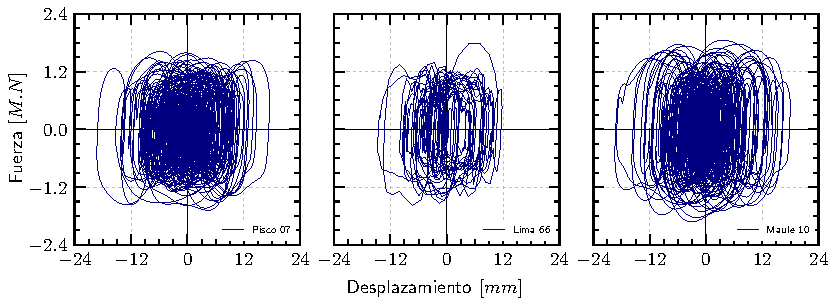
\includegraphics[scale=1]{E. Imágenes/Anexos/Anexo_1.pdf}
	\vspace{-8 mm}
	\caption[]{\centering\footnotesize Histéresis del DFV del edificio del aeropuerto Jorge Chavez.}
	\label{Anexo_1}
	\end{figure}	


	\begin{figure}[!h]
	\centering
	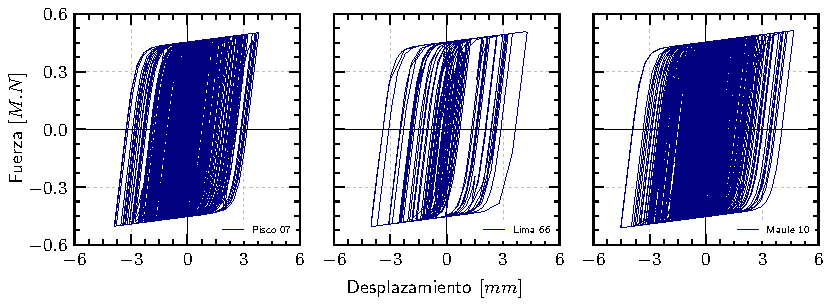
\includegraphics[scale=1]{E. Imágenes/Anexos/Anexo_2.pdf}
	\vspace{-8 mm}
	\caption[]{\centering\footnotesize Histéresis del DH-SLB del edificio del aeropuerto Jorge Chavez.}
	\label{Anexo_2}
	\end{figure}	





	
\end{document}